%%
%% Copyright 2026 Elsevier Ltd
%%
%% This file is part of the 'Elsarticle Bundle'.
%% ---------------------------------------------
%%
%% It may be distributed under the conditions of the LaTeX Project Public
%% License, either version 1.2 of this license or (at your option) any
%% later version.  The latest version of this license is in
%%    http://www.latex-project.org/lppl.txt
%% and version 1.2 or later is part of all distributions of LaTeX
%% version 1999/12/01 or later.
%%
%% The list of all files belonging to the 'Elsarticle Bundle' is
%% given in the file `manifest.txt'.
%%

%% Template article for Elsevier's document class `elsarticle'
%% with numbered style bibliographic references
%% SP 2008/03/01

\documentclass[preprint,12pt, a4paper]{elsarticle}

%% Use the option review to obtain double line spacing
%% \documentclass[authoryear,preprint,review,12pt]{elsarticle}

%% For including figures, graphicx.sty has been loaded in
%% elsarticle.cls. If you prefer to use the old commands
%% please give \usepackage{epsfig}

%% The amssymb package provides various useful mathematical symbols
\usepackage{amssymb}
\usepackage{amsmath}
\usepackage[T1]{fontenc}
\usepackage[utf8]{inputenc}
\usepackage[british]{babel}
\usepackage{booktabs}
\usepackage{xcolor}
\usepackage{tikz}
\usetikzlibrary{positioning,fit,arrows.meta,backgrounds}
\usepackage{hyperref}
\setlength{\parindent}{0pt}
%% The amsthm package provides extended theorem environments
%% \usepackage{amsthm}

%% The lineno packages adds line numbers. Start line numbering with
%% \begin{linenumbers}, end it with \end{linenumbers}. Or switch it on
%% for the whole article with \linenumbers.
%\usepackage{lineno}

%% Data that the authors still have to provide are marked in red
\newcommand{\todo}[1]{\textcolor{red}{[#1]}}
\DeclareUrlCommand\file{\urlstyle{tt}}

\journal{SoftwareX}

\begin{document}
\renewcommand{\labelenumii}{\arabic{enumi}.\arabic{enumii}}

\begin{frontmatter}

\title{Aspa: An offline tool to generate, read and grade versioned and personalised multiple-choice exams}

\author[uca]{Lorena Gutiérrez-Madroñal\corref{cor1}}
\ead{lorena.gutierrez@uca.es}
\author[uca]{Rubén Baena-Pérez}
\author[uca]{José Miguel Mota-Macías}
\cortext[cor1]{Corresponding author.}

\address[uca]{Department of Computer Science and Engineering, School of Engineering, University of Cádiz, Avda.\ de la Universidad de Cádiz 10, 11519 Puerto Real, Cádiz, Spain \todo{check department and address}}

\begin{abstract}
Paper-based multiple-choice exams remain common in higher education, but grading them requires either proprietary optical readers or tools that demand \LaTeX{} or command-line skills. Aspa is a local web application that covers the whole cycle: it builds several versions of an exam from a spreadsheet question bank, prints answer sheets with fiducial markers and a QR code, reads scans or mobile-phone photographs with computer vision, grades them with configurable negative marking and partial credit, and supports reviewing each sheet with the student. It can also produce personalised exams that omit the questions each student has already passed during the course. Everything runs on the teacher's computer, so students' data never leave it.
\end{abstract}

\begin{keyword}
Multiple-choice exams \sep Optical mark recognition \sep Automated grading \sep Personalised assessment \sep Continuous assessment \sep Higher education
\end{keyword}

\end{frontmatter}

%\linenumbers

\section*{Required Metadata}
\label{sec:metadata}

\section*{Current code version}
\label{sec:codeversion}

\begin{table}[!h]
\begin{tabular}{|l|p{5.6cm}|p{6.4cm}|}
\hline
\textbf{Nr.} & \textbf{Code metadata description} & \textbf{Please fill in this column} \\
\hline
C1 & Current code version & v1.0.0 \\
\hline
C2 & Permanent GitHub link to code/repository used for this code version & \url{https://github.com/lorenagmad/Aspa} \\
\hline
C3 & Legal Code License   & GNU Affero General Public License v3.0 or later (AGPL-3.0-or-later) \\
\hline
C4 & Code versioning system used & git \\
\hline
C5 & Software code languages, tools, and services used & Python 3; Flask, OpenCV, NumPy, ReportLab, openpyxl, PyMuPDF; HTML, CSS and JavaScript (Jinja2 templates, SVG) \\
\hline
C6 & Compilation requirements, operating environments \& dependencies & Python $\geq$ 3.9 on Windows, macOS or Linux; dependencies in \file{requirements.txt}, installed automatically by the launch scripts; any modern web browser. No internet connection needed after installation. \\
\hline
C7 & If available Link to developer documentation/manual & \url{https://github.com/lorenagmad/Aspa\#readme} (help pages are also built into the application) \\
\hline
C8 & Support email for questions & \href{mailto:lorena.gutierrez@uca.es}{lorena.gutierrez@uca.es} \\
\hline
\end{tabular}
\caption{Code metadata (mandatory)}
\label{tab:codemetadata}
\end{table}

%% ============================================================================
\section{Motivation and significance}
\label{sec:motivation}

Multiple-choice questions (MCQs) are one of the most widely used assessment formats in higher education because they sample a large part of a syllabus in little time and can be graded objectively~\cite{haladyna2002}. When exams are taken on paper, which is still the norm in many examination halls, grading a large group by hand is slow and error-prone, and the item analysis that would allow a teacher to detect badly worded questions or wrong answer keys~\cite{ebel1991} is rarely carried out. Practices that improve the reliability and fairness of the exam, such as distributing several versions of the same exam so that neighbouring students receive different questions or orderings, or applying negative marking to discourage guessing~\cite{burton2005}, make manual grading even more laborious.

Continuous assessment introduces an additional requirement. Many courses combine frequent low-stakes quizzes, which are known to improve retention~\cite{roediger2006} and to provide formative feedback~\cite{black1998,hattie2007}, with a final exam. A natural policy in this setting, inspired by mastery learning~\cite{bloom1968}, is to exempt each student from the final-exam questions whose content they have already demonstrated during the term. Applying such a policy on paper means producing a different exam for every student and grading each one against its own key, which is impractical without software support.

Several tools address part of this problem. Commercial optical mark recognition (OMR) products such as Remark OMR or the ZipGrade mobile app~\cite{zipgrade} read answer sheets but are proprietary, and cloud-based solutions upload students' personal data to third-party servers, which is problematic under the European General Data Protection Regulation~\cite{gdpr}. Open-source alternatives exist: Auto Multiple Choice (AMC)~\cite{amc} is a mature and powerful system, but exams are written in \LaTeX{} and it runs on Linux and macOS only; the R/exams package~\cite{zeileis2014} generates exams from R or Markdown sources and can scan its own sheets, but requires R programming skills; FormScanner~\cite{formscanner} and OMRChecker~\cite{omrchecker} read generic bubble sheets but neither generate exams nor grade them with versions, partial credit or student review. To the best of our knowledge, none of them supports exams personalised per student from a record of the questions passed in class.

Aspa was developed by the authors to grade their own exams at the University of Cádiz, and was designed around three requirements: (i)~a teacher with no programming knowledge must be able to use it with the files they already have (a question bank and the class list exported from the university system, both as spreadsheets); (ii)~it must read sheets digitised in any available way, from a sheet-fed office scanner to a photograph taken with a mobile phone; and (iii)~all data must remain on the teacher's computer. Its typical use is depicted in the six steps of the application: upload the question bank and the class list; configure the exam (type, language, scoring and versions); generate the PDF to print; drag the scans into the browser, where they are read and graded automatically and every doubtful case is flagged for review; inspect the item statistics, voiding questions or correcting keys if necessary; and export the grades to Excel. Beyond grading, the per-question data it collects (the distribution of the options chosen in every question and version) make it a convenient instrument for research on item quality, negative marking and personalised assessment.

%% ============================================================================
\section{Software description}
\label{sec:description}

Aspa (version 1.0.0) is written in Python and runs as a local web application: a Flask server bound to \file{127.0.0.1} serves the interface to the teacher's browser, which opens automatically. Double-clickable launch scripts for Windows, macOS and Linux create a virtual environment and install the dependencies on the first run, and a script based on PyInstaller builds a single executable that does not need Python. The interface is available in Spanish and English, and new languages are added with a JSON file.

\subsection{Software architecture}
\label{sec:architecture}

Figure~\ref{fig:architecture} shows the components. The web layer (\file{app.py}, Jinja2 templates and a small amount of JavaScript for the review screen) contains no exam logic, which lives in the \file{examtool} package. Two design decisions shape the architecture.

\begin{figure}[t]
\centering
\resizebox{\textwidth}{!}{%
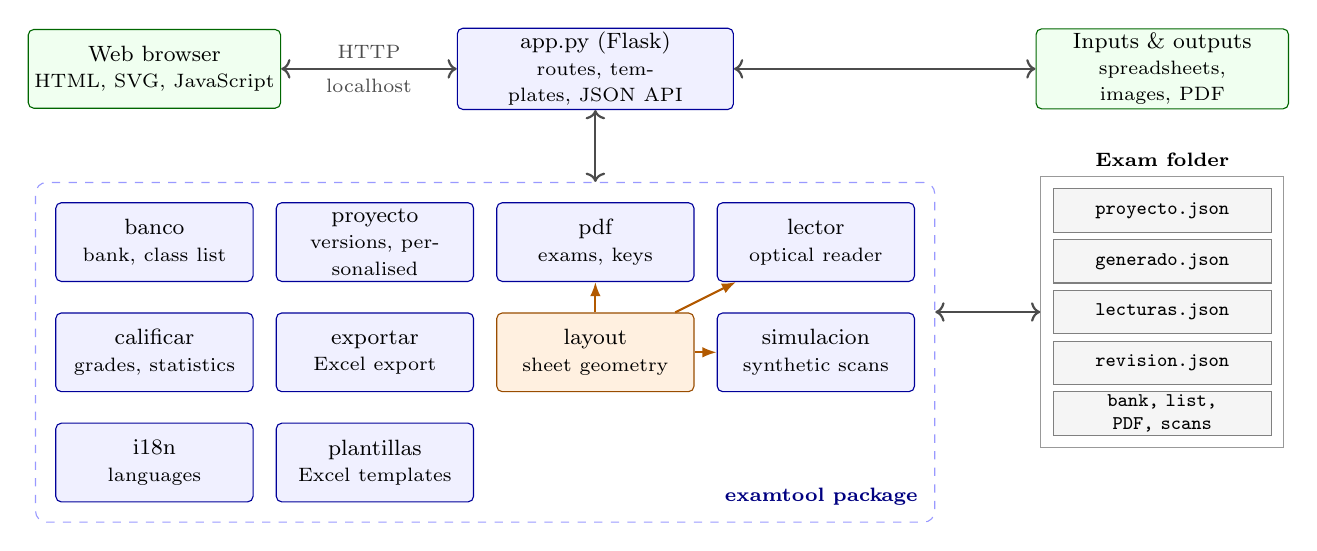
\begin{tikzpicture}[x=1mm, y=1mm, font=\footnotesize,
  mod/.style={draw=blue!60!black, fill=blue!6, rounded corners=2pt, align=center, minimum height=10mm, text width=24mm, inner sep=1.5pt},
  dat/.style={draw=black!50, fill=black!4, align=center, minimum height=5.5mm, text width=27mm, inner sep=1pt, font=\scriptsize\ttfamily},
  ext/.style={draw=green!40!black, fill=green!6, rounded corners=2pt, align=center, minimum height=10mm, text width=31mm, inner sep=1.5pt},
  arr/.style={-{Latex[length=1.8mm]}, thick, black!70}]
  % web layer
  \node[ext] (browser) at (0,22) {Web browser\\ \scriptsize HTML, SVG, JavaScript};
  \node[mod, text width=34mm] (app) at (56,22) {\file{app.py} (Flask)\\ \scriptsize routes, templates, JSON API};
  \node[ext] (files) at (128,22) {Inputs \& outputs\\ \scriptsize spreadsheets, images, PDF};
  % core modules (4 columns x 3 rows)
  \node[mod] (banco)     at (0,0)    {\file{banco}\\ \scriptsize bank, class list};
  \node[mod] (proyecto)  at (28,0)   {\file{proyecto}\\ \scriptsize versions, personalised};
  \node[mod] (pdf)       at (56,0)   {\file{pdf}\\ \scriptsize exams, keys};
  \node[mod] (lector)    at (84,0)   {\file{lector}\\ \scriptsize optical reader};
  \node[mod] (calificar) at (0,-14)  {\file{calificar}\\ \scriptsize grades, statistics};
  \node[mod] (exportar)  at (28,-14) {\file{exportar}\\ \scriptsize Excel export};
  \node[mod, fill=orange!12, draw=orange!60!black] (layout) at (56,-14) {\file{layout}\\ \scriptsize sheet geometry};
  \node[mod] (simul)     at (84,-14) {\file{simulacion}\\ \scriptsize synthetic scans};
  \node[mod] (i18n)      at (0,-28)  {\file{i18n}\\ \scriptsize languages};
  \node[mod] (plant)     at (28,-28) {\file{plantillas}\\ \scriptsize Excel templates};
  \begin{scope}[on background layer]
    \node[draw=blue!40, dashed, rounded corners, fit=(banco)(lector)(i18n)(simul), inner sep=2.5mm] (pkg) {};
  \end{scope}
  \node[font=\scriptsize\bfseries, blue!50!black, anchor=south east] at ([xshift=-1mm, yshift=1mm]pkg.south east) {\file{examtool} package};
  % exam folder
  \node[dat] (cfg)  at (128,4)   {proyecto.json};
  \node[dat, below=0.8mm of cfg] (gen)  {generado.json};
  \node[dat, below=0.8mm of gen] (lect) {lecturas.json};
  \node[dat, below=0.8mm of lect] (rev) {revision.json};
  \node[dat, below=0.8mm of rev] (scans) {bank, list, PDF, scans};
  \node[draw=black!40, fit=(cfg)(scans), inner sep=1.5mm] (folder) {};
  \node[font=\scriptsize\bfseries, anchor=south] at (folder.north) {Exam folder};
  % arrows
  \draw[arr, <->] (browser) -- node[above, font=\scriptsize]{HTTP} node[below, font=\scriptsize]{localhost} (app);
  \draw[arr, <->] (app) -- (files);
  \draw[arr, <->] (app) -- (pkg.north -| app);
  \draw[arr, orange!70!black] (layout) -- (pdf);
  \draw[arr, orange!70!black] (layout) -- (lector);
  \draw[arr, orange!70!black] (layout) -- (simul);
  \draw[arr, <->] (pkg.east |- lect) -- (folder.west |- lect);
\end{tikzpicture}}
\caption{Architecture of Aspa. The geometry of the answer sheet (\texttt{layout}, orange) is shared by the PDF generator, the reader and the simulator. Each exam is a folder of plain files; grades are never stored but recomputed from the readings, the manual revisions and the settings.}
\label{fig:architecture}
\end{figure}

First, a single module, \file{layout}, defines the geometry of the answer sheet in millimetres. It is used by the PDF generator (ReportLab), by the optical reader (OpenCV~\cite{opencv}) and by a scan simulator, so a change in the design of the sheet cannot leave the generator and the reader out of step.

Second, each exam is a self-contained folder of human-readable files: the editable settings (\file{proyecto.json}), the question bank and the class list, the versions frozen at generation time (\file{generado.json}: random seed, order of questions and options of every version, answer keys and a copy of the bank), the scans, what the reader found on each page (\file{lecturas.json}) and the teacher's manual corrections (\file{revision.json}). Grades are never stored: they are computed as a pure function of readings, revisions, frozen versions and settings. Consequently, changing the penalty for wrong answers, voiding a question or correcting an answer key updates every grade at once, and re-reading all the scans with a new version of the reader never overwrites the corrections the teacher has made. Files are written atomically, and deleting an exam only moves its folder to a recycle bin.

\subsection{Software functionalities}
\label{sec:functionalities}

\paragraph{Question bank and class list} The bank is a spreadsheet (Excel or CSV) with one row per question: identifier, topic, stem, up to four options, correct letters (\texttt{B}, \texttt{AC}\dots, or digits as in legacy banks), group, fixed options and an optional explanation of the correct answer. Column headers are recognised by synonyms in Spanish and English. Questions may have several correct answers, fewer than four options (e.g.\ true/false) and options that must not move when shuffling; options beginning with phrases such as ``All of the above'' or ``None of the above'' are fixed automatically. Duplicate identifiers, empty keys and keys that point to empty options produce warnings. The class list accepts the format exported by the university system, a simple \emph{document--name} sheet or a sheet with the questions each student has passed. Blank templates, templates with commented examples and help pages are available from the home screen.

\paragraph{Exam versions} Each version (A, B, C\dots) lists the question groups it draws from; if they do not provide enough questions, the rest are chosen at random among the ungrouped questions, and a version without groups samples the whole bank. Before generating, Aspa reports for every version how many questions come from its groups and how many at random, or how many are missing (Figure~\ref{fig:screens}a). Questions and options are shuffled in each version with a recorded seed. The PDF contains all the copies, interleaved (A, B, C, D, A\dots) so that neighbouring students receive different versions, with a blank page added where needed for duplex printing; images referenced by the questions are printed at the end with their captions. A second PDF gives the key of each version and the correspondence between printed and bank questions. Regenerating an exam once scans have been read requires explicit confirmation, since it would invalidate the printed copies.

\paragraph{Personalised exams} In this mode each student on the list receives their own exam with their name and identity document printed on the sheet and without the questions they have already passed in class, which count as correct (Figure~\ref{fig:sheets}b). Each student is assigned to a version whose pool contains all their passed questions, balancing the number of students per version; their exam consists of the questions of that pool minus the passed ones. Spare, non-personalised copies are generated for students not on the list.

\paragraph{Answer sheet} The first page of every copy is the answer sheet (Figure~\ref{fig:sheets}a). Four ArUco fiducial markers~\cite{garrido2014} delimit the reading area; a QR code encodes the exam code, version, copy number and, in personalised exams, the student's document; a grid of ten columns of digits records the identity document, so that Spanish national identity cards, residence cards and passports can be used (only their digits are compared); answers are marked in boxes A--D, up to 30 questions per sheet; and a separate \emph{Cancel} box per question, together with a free-text box, lets students void or change an answer. Instructions are generated in the language of the exam, which is independent of the language of the interface.

\begin{figure}[!htb]
\centering
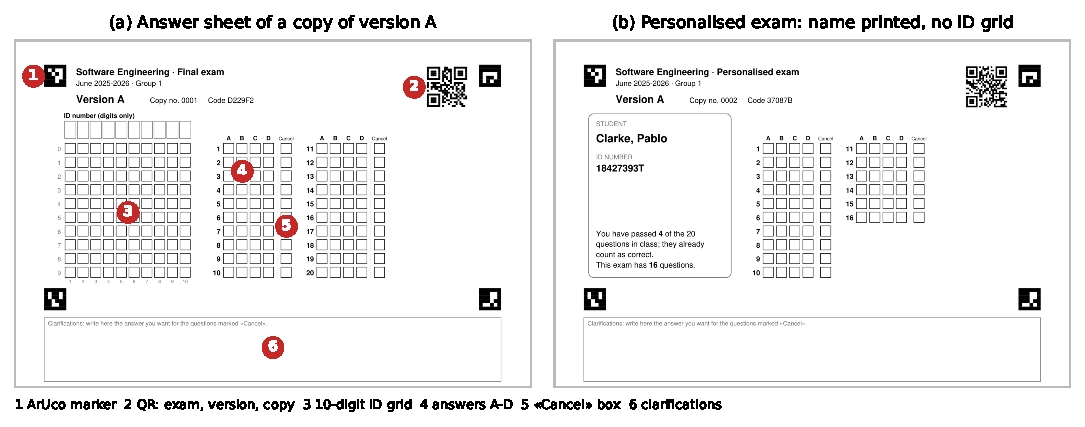
\includegraphics[width=\textwidth]{figures/fig_sheets.pdf}
\caption{Printed exams. (a)~Answer sheet at the top of the first page of a copy of version~A; the instructions and the questions follow below it. (b)~Answer sheet of a personalised exam: the student's name and document replace the identity grid, and the sheet states that four of the twenty questions were passed in class, so only sixteen boxes are printed.}
\label{fig:sheets}
\end{figure}

\paragraph{Optical mark recognition} Scans can be images (JPEG, PNG, TIFF\dots) or multi-page PDF files, which are rasterised at 220~dpi with PyMuPDF. For each page the reader (Figure~\ref{fig:pipeline}):
(1)~detects the ArUco markers, retrying with contrast enhancement (CLAHE) if fewer than three are found, and estimates with RANSAC the homography that maps the page onto the template, which corrects rotation (including sheets fed upside down), scale and perspective; three markers suffice;
(2)~rectifies the page at 8~pixels/mm and normalises the illumination by dividing it by an estimate of the paper background (a morphological closing with a 7~mm kernel followed by Gaussian smoothing), which removes shadows and uneven scanner lighting;
(3)~decodes the QR code from its expected region, enlarged and binarised if necessary;
(4)~locates the printed boxes, because a homography cannot model paper curvature or lens distortion, which may shift a block of boxes by 1--2~mm: square contours of the size of a box are detected, and each block (the identity grid and each column of ten questions) is fitted to them with a robust median shift, an affine transformation estimated with RANSAC, and a final snap of each box to the nearest printed box;
(5)~measures the fraction of ink pixels inside each box, leaving a margin to exclude the printed border, and classifies it with thresholds adapted to the sheet: a box is marked if its ratio exceeds $\max(0.11,\, m+0.10)$ and doubtful if it exceeds $\max(0.04,\, m+0.04)$, where $m$ is the median ratio of the printed boxes, which are mostly empty, so that thick printing or grey paper do not create false marks.
Blank pages and pages without markers (e.g.\ the question pages of a duplex scan) are ignored. Reading runs in a background thread while the browser shows its progress.

\begin{figure}[!htb]
\centering
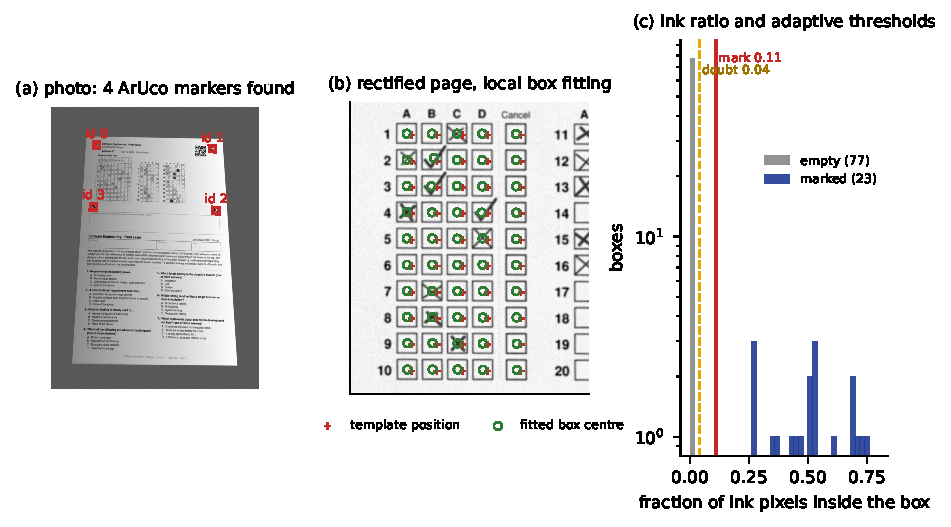
\includegraphics[width=\textwidth]{figures/fig_pipeline.pdf}
\caption{Reading a synthetic phone photograph (keystone distortion, 1.6~mm paper warping, shadow, blur and JPEG compression). (a)~The four markers are detected. (b)~After rectification and illumination normalisation, the template positions of the boxes (red crosses) are up to 1.3~mm away from the printed boxes; the local fitting places the measurement on them (green circles). (c)~Fraction of ink in each answer box: empty and marked boxes are clearly separated by the adaptive thresholds. All 20 answers, the QR code and the identity document were read correctly.}
\label{fig:pipeline}
\end{figure}

\paragraph{Identification and incidences} The digits read from the grid are matched with the class list, ignoring leading zeros. Columns with more than one mark act as wildcards, faint marks are accepted but flagged, and a unique student whose document differs in a single digit is proposed, in both cases flagged for checking. Each sheet ends up \emph{correct}, \emph{to review} or \emph{unreadable}, and the reasons are listed: QR code from another exam or unreadable, document not on the list or not marked, doubtful digits or marks, \emph{Cancel} boxes pending review, or the same student on two sheets.

\paragraph{Grading} With $b$ points for a correct answer and $w<0$ for a wrong one, a question whose key is the set $C$ and on which the student marked the set $M$ scores $0$ if $M=\varnothing$, $b$ if $M=C$, and $w$ otherwise when $|C|=1$. For multiple-answer questions in the default \emph{partial credit} mode, with $h=|M\cap C|$ hits and $e=|M\setminus C|$ errors, the score is $w$ if $h=0$ and $b\cdot\max(0,h-e)/|C|$ otherwise; in \emph{exact} mode anything but $M=C$ scores $w$ (Table~\ref{tab:scoring}). A marked \emph{Cancel} box leaves the question at zero until the teacher reads the clarification and enters the intended answer. The grade is the total divided by the maximum attainable on the valid questions and scaled to the chosen maximum (10 by default); voided questions leave the denominator, questions passed in class add $b$, and negative final grades are optional.

\begin{table}[t]
\centering
\caption{Score of a question whose correct answers are A and B ($b=1$, $w=-0.25$) for several sets of marks, as computed by Aspa in both modes.}
\label{tab:scoring}\vspace{3pt}
\small\setlength{\tabcolsep}{4pt}
\begin{tabular}{lccccccccc}
\toprule
Marked & AB & A & B & ABC & AC & ABCD & C & CD & (blank) \\
\midrule
Partial credit & 1 & 0.5 & 0.5 & 0.5 & 0 & 0 & $-0.25$ & $-0.25$ & 0 \\
Exact & 1 & $-0.25$ & $-0.25$ & $-0.25$ & $-0.25$ & $-0.25$ & $-0.25$ & $-0.25$ & 0 \\
\bottomrule
\end{tabular}
\end{table}

\paragraph{Review} The review screen (Figure~\ref{fig:review}) superimposes the result on the rectified scan, drawn on the boxes actually located by the reader: marked and correct, marked and wrong, correct but not marked, and \emph{Cancel} or doubtful marks have distinct colours. Clicking a box or editing the table changes the answer and recalculates the grade instantly; the teacher can also assign the sheet to another student with a searchable list, override the version given by the QR code, mark the sheet as reviewed, open the original scan and move between sheets with the arrow keys. Hovering over a question shows its text, the options chosen and, if the student did not answer it correctly and the bank provides one, the explanation of the correct answer; explanations may be added to the bank after the exam. A \emph{review with the student} mode hides all editing controls so that the screen can be shown during the exam review.

\begin{figure}[!htb]
\centering
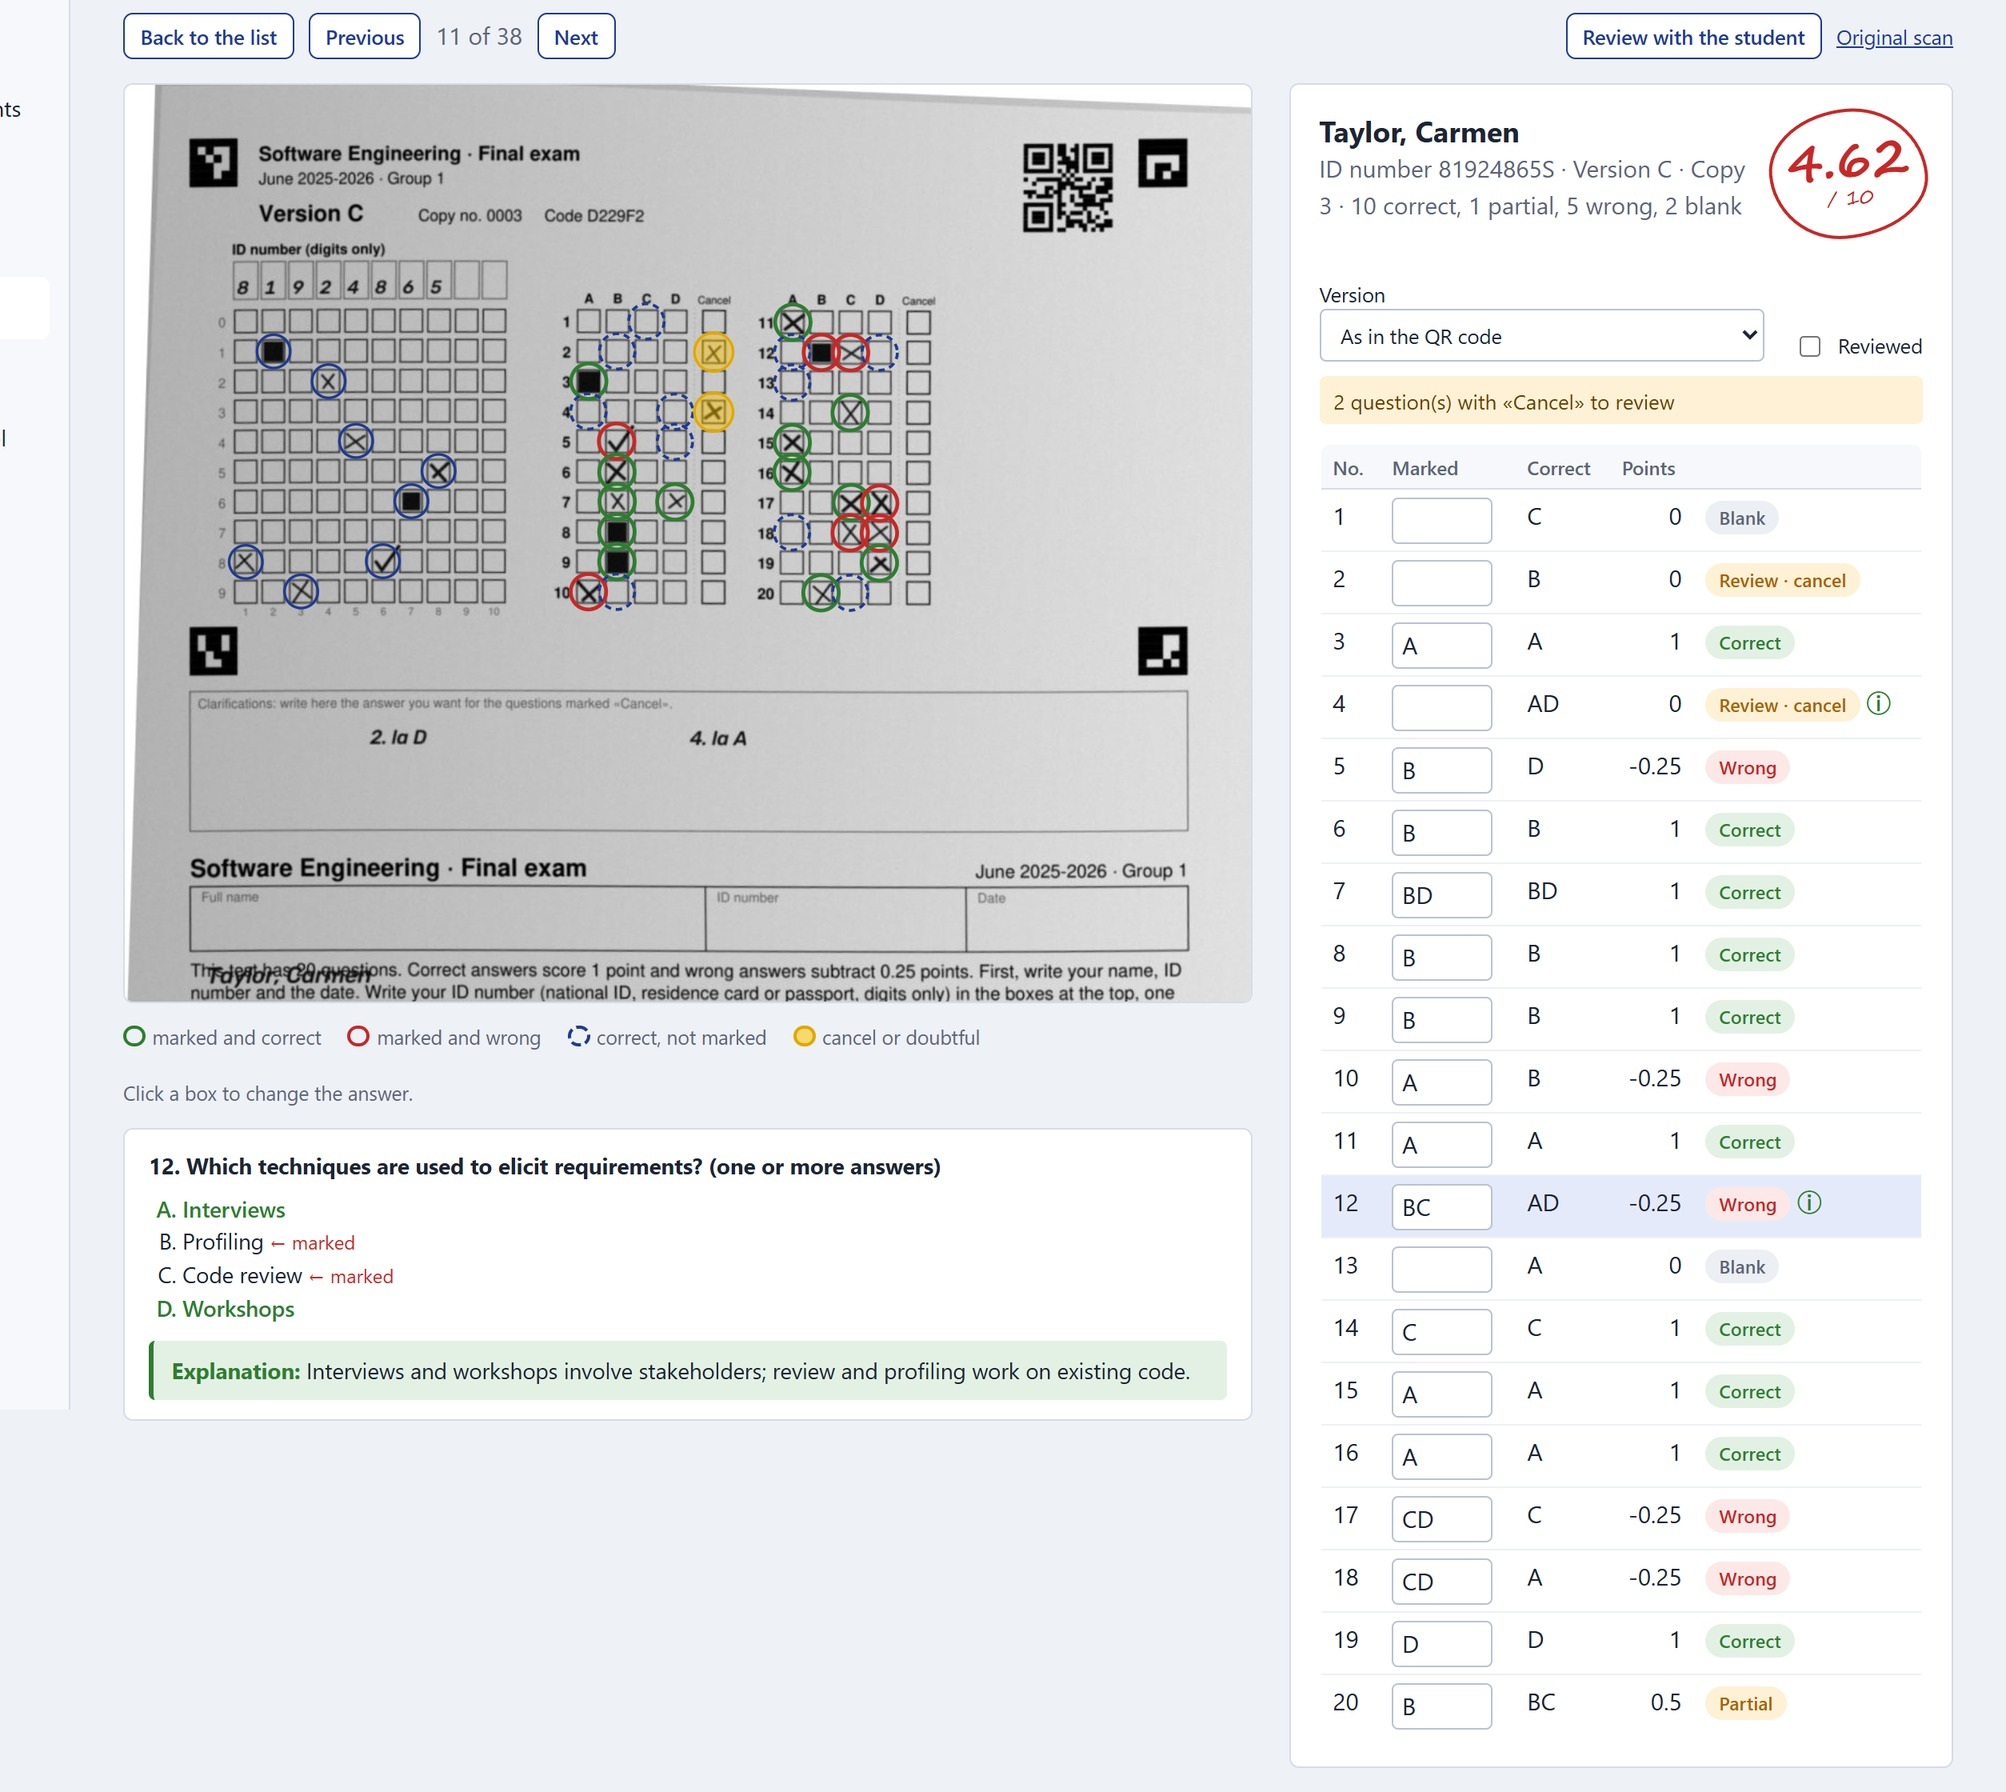
\includegraphics[width=\textwidth]{figures/fig_review.jpg}
\caption{Review screen. The result is drawn on the rectified scan (green: marked and correct; red: marked and wrong; dashed blue: correct but not marked; yellow: \emph{Cancel} box). The student cancelled questions 2 and 4 and wrote the intended answers in the clarifications box, so the sheet is pending review. On the right, the student identified from the ID grid, the grade and the editable table; below the sheet, the hovered question~12 with the options marked and the explanation of the correct answer.}
\label{fig:review}
\end{figure}

\paragraph{Item statistics and adjustments} For every bank question used, Aspa reports how many students received it, the success rate, the mean score and how many chose each option, expressed in the order of the bank so that versions can be compared (Figure~\ref{fig:screens}b). Questions are sorted from lowest to highest success rate, which brings questions with a wrong key or ambiguous wording to the top. A question can be voided for everyone or given a corrected key, which Aspa maps onto the shuffled order of each version; all grades are recalculated immediately and remain reversible.

\begin{figure}[!htb]
\centering
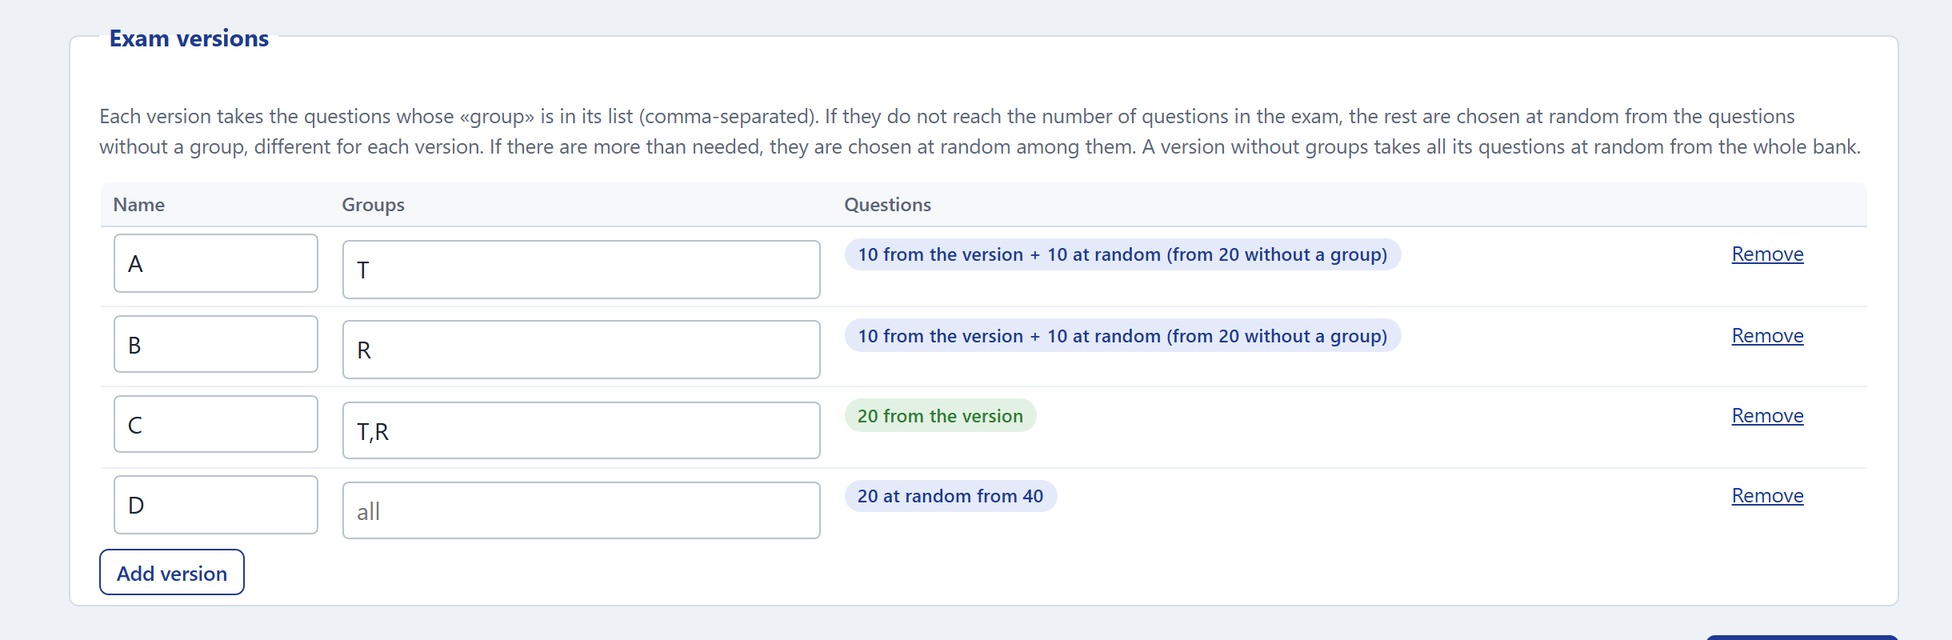
\includegraphics[width=0.92\textwidth]{figures/fig_versions.jpg}\\[1mm]
{\footnotesize (a)}\\[2mm]
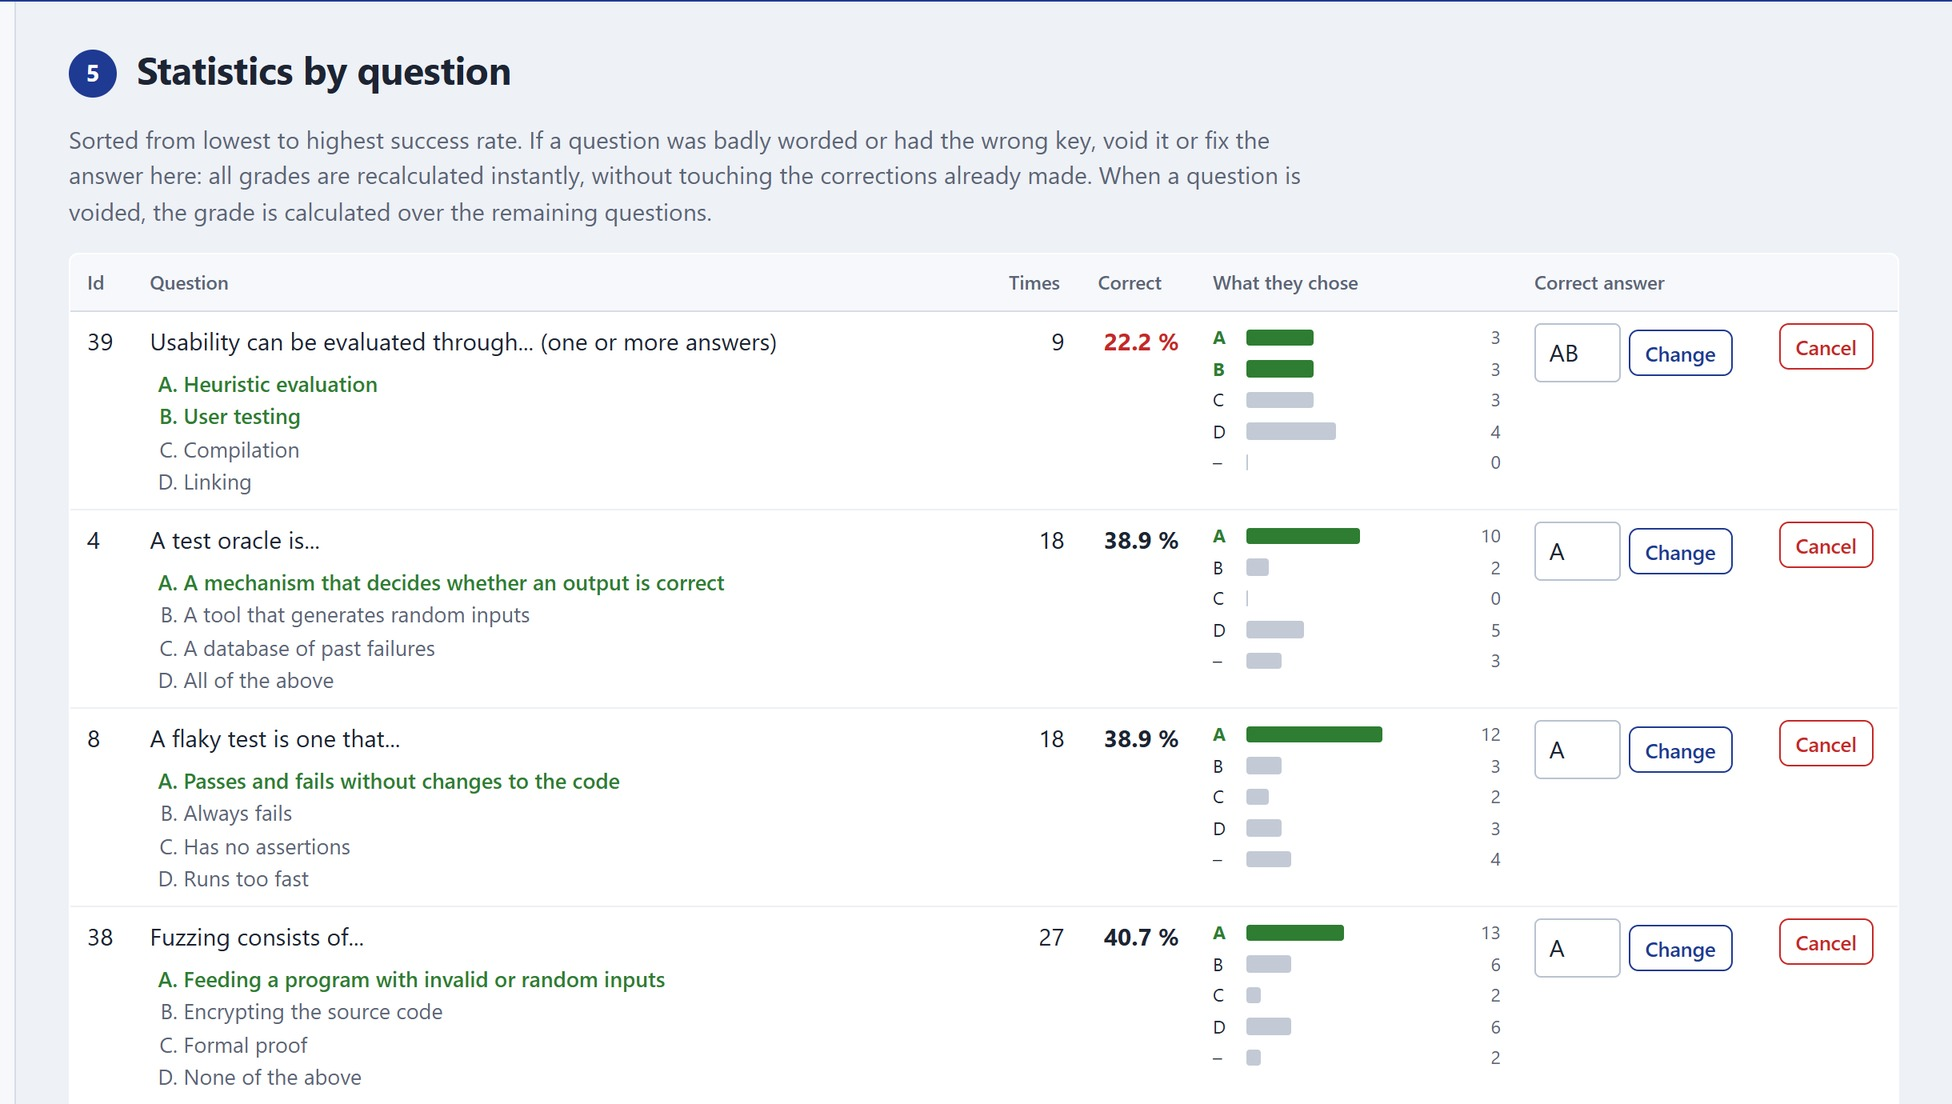
\includegraphics[width=0.92\textwidth]{figures/fig_statistics.jpg}\\[1mm]
{\footnotesize (b)}
\caption{(a)~Configuration of the four versions of the example and the check of where their questions come from. (b)~Item statistics, sorted by success rate: options chosen (correct ones in green, expressed in the order of the bank), corrected key and voiding of each question.}
\label{fig:screens}
\end{figure}

\paragraph{Export and organisation} Grades are exported to an Excel workbook with six sheets: grades with the incidences (sheets pending review highlighted), the class list with absent students marked, answers, points per bank question, item statistics and the settings used. The home screen lists the exams with filters by subject, session, academic year and status; a new exam can start from a previous one, copying its bank, class list and settings.

\subsection{Sample code snippets analysis}
\label{sec:snippets}

The core can also be used from Python, which is how the experiments of Section~\ref{sec:examples} were run. The following lines generate a project, read a folder of scans and export the grades:

{\footnotesize
\begin{verbatim}
from examtool.proyecto import Proyecto
from examtool.pdf import generar_pdf, generar_soluciones
from examtool.lector import leer_proyecto
from examtool.exportar import exportar_excel

p = Proyecto("ExamenesTest/final-exam")   # folder with bank and class list
p.generar(semilla=2026); generar_pdf(p); generar_soluciones(p)
leer_proyecto(p)                          # reads every file in escaneos/
exportar_excel(p)                         # writes notas.xlsx
\end{verbatim}
}

The repository also provides tools to test the reader without printing. The script \file{herramientas/simular_escaneos.py} fills the sheets of a generated exam with known answers in several styles (crosses, filled boxes, ticks, light pencil, stray marks, voided answers) and degrades them as a scanner or a phone camera would, and \file{herramientas/evaluar_simulacion.py} compares what is read with the ground truth.

%% ============================================================================
\section{Illustrative examples}
\label{sec:examples}

\subsection{A complete exam}

We illustrate Aspa with a 40-question bank on software engineering (\emph{testing} questions in group T, \emph{requirements} in group R and 20 ungrouped questions, including multiple-answer, true/false and fixed-order questions) and a fictitious class of 40 students with national identity, residence card and passport numbers. The data and every script used in this section are in the \file{SoftwareX/experiments} folder of the repository, so the results can be reproduced.

Four versions of 20 questions were configured: A (group T plus ten random ungrouped questions), B (group R plus ten), C (groups T and R) and D (twenty questions from the whole bank) (Figure~\ref{fig:screens}a). Generating the 40 copies (160 duplex pages) and the answer keys took 3.3~s. Thirty-six copies were then filled in by the simulator and degraded; thirty were uploaded as JPEG images and six inside a single PDF that also contained a blank page and a question page, as a sheet-fed scanner would produce. The 38 pages were read in 11.5~s on a laptop computer \todo{processor model}: the two extra pages were ignored, the 720 answers were read without error, and all 36 students were identified. Twenty-one sheets were flagged for review, all because of \emph{Cancel} boxes that the simulator had marked on purpose; Figure~\ref{fig:review} shows one of them during review, with question~12 selected to display its explanation.

On the statistics screen (Figure~\ref{fig:screens}b), voiding the question with the lowest success rate changed 18 grades at once while preserving the manual corrections, and correcting a key was correctly translated into the printed order of each version; restoring them restored the original grades. The same exam was then created in a personalised version from a class list in which students had passed between 0 and 6 of the ten questions of their version's group: Aspa produced 40 personalised exams with 14 to 20 questions and 3 spare copies, identified every sheet from its QR code, and counted the passed questions as correct.

These steps belong to an end-to-end test suite that drives the web interface as a teacher would, covering also the templates and help pages, parsing of legacy banks and CSV files, student matching, both scoring modes, regeneration protection, copying an exam, the recycle bin, exporting and the independence of exam and interface languages. All 67 checks passed.

\subsection{Reading accuracy and robustness}
\label{sec:accuracy}

To quantify the reader we filled sheets with known answers (10\% blank, 50\% correct, 15\% two options, the rest a single random option, and 5\% \emph{Cancel} marks; crosses, filled boxes and ticks) and read them with the same function Aspa applies to a real scan. In the first experiment, 500 sheets were degraded with a random mixture of defects: rotation of up to $\pm 4^\circ$ (one sheet in ten upside down), perspective, non-linear warping of up to 2~mm, a lateral shadow, grey paper, noise, blur and JPEG compression, with ink ranging from a black pen to a light pencil (grey level 130 on 255). Table~\ref{tab:accuracy} summarises the results. Of the 9,940 answers on the sheets that were read, only one was misread, and it was flagged as doubtful; every identity document was read correctly. The few sheets that could not be processed automatically were those in which the random displacement had pushed part of the page out of the image: with two markers missing, Aspa reports that the sheet seems cropped and asks for it to be rescanned, and with the QR code cut off it asks the teacher to choose the version. Reading took 0.21~s per page on average.

\begin{table}[t]
\centering
\caption{Reading of 500 synthetic sheets with mixed defects (exam with versions) and 125 personalised sheets. Unread sheets are reported to the teacher with the reason; flagged errors are shown as doubtful in the review screen.}
\label{tab:accuracy}\vspace{3pt}
\begin{tabular}{lcc}
\toprule
 & Versions & Personalised \\
\midrule
Sheets & 500 & 125 \\
Sheets read (others reported as cropped) & 497 (99.4\%) & 123 (98.4\%) \\
QR code decoded & 496 (99.2\%) & 123 (98.4\%) \\
Identity document read correctly & 497/497 (100\%) & --- (printed) \\
Answers read exactly (on sheets read) & 9,939/9,940 & 2,126/2,126 \\
\quad Errors flagged as doubtful & 1/1 & --- \\
False marks / missed marks & 0 / 1 & 0 / 0 \\
Mean reading time per page & 0.21~s & 0.15~s \\
\bottomrule
\end{tabular}
\end{table}

In the second experiment each defect was varied separately on 30 sheets per level, adding mild noise (Figure~\ref{fig:robustness}). All answers, documents and QR codes were read correctly at any rotation (including 90$^\circ$, 180$^\circ$ and 270$^\circ$), with random corner displacements of up to 10\% of the page width, with phone keystone distortion of up to 30\%, with JPEG quality as low as 5, with noise of up to 40 grey levels, with shadows that darken one side of the page to 20\% of its brightness, and with one marker covered. Accuracy remained at 100\% down to 120~dpi and above 99.6\% down to 60~dpi, with every error flagged. The limits are reached with paper warping of more than 2~mm, which exceeds the tolerance of the local box fitting, blur beyond a Gaussian of 2~pixels at 220~dpi (about 0.25~mm, an out-of-focus photograph) and very faint marks: ink lighter than 66\% of the brightness of the paper (grey level 175 in the experiment) is not detected, in which case the sheet is flagged because no identity document is found. In practice, it is therefore advisable to scan at 150--300~dpi or take sharp, well-framed photographs, and mark with a pen or a soft pencil.

\begin{figure}[t]
\centering
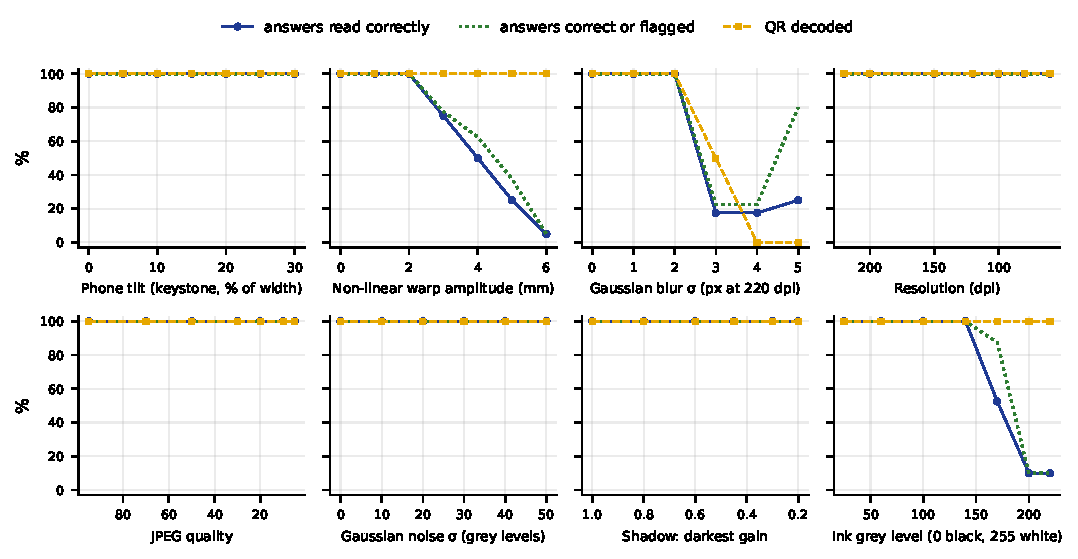
\includegraphics[width=\textwidth]{figures/fig_robustness.pdf}
\caption{Robustness of the reader to individual defects (30 sheets per level, 600 answers). Solid: answers read exactly; dotted: answers read exactly or flagged as doubtful for review; dashed: QR codes decoded. Resolutions refer to the scanned page; blur is measured at 220~dpi.}
\label{fig:robustness}
\end{figure}

%% ============================================================================
\section{Impact}
\label{sec:impact}

\paragraph{Daily practice} Aspa removes the manual steps between the question bank and the grades. Versions and their keys are produced from the same spreadsheet that the teacher already maintains; printed sheets can be digitised with the multi-function printer of the department or photographed with a phone; and reading a class takes seconds, so the teacher's time is spent only on the sheets that need a decision, which the program lists together with the reason. Because grades are recomputed rather than stored, decisions that are usually avoided because of their cost, such as voiding a flawed question after the exam or correcting a key, become a single click and are documented in the exported workbook. The \emph{review with the student} mode, with the question text and the explanation of the correct answer, turns the formal exam review into a feedback session~\cite{hattie2007} and makes grading transparent, which reduces disputes. Since nothing is uploaded to external services, the tool can be adopted without a data-protection impact assessment of a third-party provider~\cite{gdpr}.

\paragraph{New research questions} Personalised exams make it feasible to apply, on paper and at scale, assessment policies that reward continuous work by exempting students from the content they have already mastered~\cite{bloom1968}. This allows questions to be studied that were impractical to pursue before, for instance whether such exemptions increase participation in formative quizzes, how they affect the final grade distribution, or whether a personalised final exam measures the same construct as the complete one. The per-option, per-version responses exported by Aspa, together with the versions frozen in \file{generado.json}, also support research on item quality and distractor analysis~\cite{ebel1991}, on order effects between versions, and on negative marking and partial-credit scoring of multiple-response items~\cite{burton2005}, since grades under different scoring rules can be recomputed from the same readings.

\paragraph{Improvement of existing practice} Compared with the alternatives discussed in Section~\ref{sec:motivation}, Aspa requires neither \LaTeX{} nor programming, runs on the three major operating systems, accepts phone photographs thanks to the local alignment of the box blocks, and integrates generation, reading, review and item analysis in one tool. The scan simulator and the evaluation script make the reader testable without printing, which facilitates extending it.

\paragraph{Use} \todo{Describe the actual use: courses and degrees of the University of Cádiz in which Aspa has been used, number of exams and students graded since its first use, academic years, and any colleagues or institutions that have adopted it. Add downloads or GitHub statistics if available, and cite any publication or teaching-innovation project that has used it.} Aspa is distributed under the AGPL licence, which allows any institution to use and adapt it and requires that modified versions offered as a service publish their source code. It is not used commercially and has not led to a spin-off company.

%% ============================================================================
\section{Conclusions}
\label{sec:conclusions}

Aspa is an open-source local web application that covers the complete cycle of paper-based multiple-choice exams: generation of versions from a spreadsheet bank, personalised exams that exclude the questions each student has passed in class, robust optical reading of scans and phone photographs, grading with negative marking and partial credit, review with the student, item statistics with reversible adjustments and export to Excel. Its design keeps the sheet geometry in a single module and recomputes grades from plain files, so that settings can change after the exam without losing manual corrections. Synthetic experiments show that the reader is accurate under the defects found in practice and that its rare errors are mostly flagged for review. Future work includes evaluating the reader on a large set of real scans, supporting more than four options and 30 questions per sheet, and exporting results to learning management systems such as Moodle.

\section*{Acknowledgements}
\label{sec:acknowledgements}

\todo{Optional: thank colleagues and students who tested Aspa, and mention any funding (e.g.\ teaching-innovation projects of the University of Cádiz).}

%% References
\begin{thebibliography}{00}

\bibitem{haladyna2002} T.~M. Haladyna, S.~M. Downing, M.~C. Rodriguez, A review of multiple-choice item-writing guidelines for classroom assessment, Applied Measurement in Education 15~(3) (2002) 309--333. \url{https://doi.org/10.1207/S15324818AME1503_5}

\bibitem{ebel1991} R.~L. Ebel, D.~A. Frisbie, Essentials of Educational Measurement, 5th ed., Prentice Hall, Englewood Cliffs, NJ, 1991.

\bibitem{burton2005} R.~F. Burton, Multiple-choice and true/false tests: myths and misapprehensions, Assessment \& Evaluation in Higher Education 30~(1) (2005) 65--72. \url{https://doi.org/10.1080/0260293042003243904}

\bibitem{roediger2006} H.~L. Roediger, J.~D. Karpicke, Test-enhanced learning: taking memory tests improves long-term retention, Psychological Science 17~(3) (2006) 249--255. \url{https://doi.org/10.1111/j.1467-9280.2006.01693.x}

\bibitem{black1998} P.~Black, D.~Wiliam, Assessment and classroom learning, Assessment in Education: Principles, Policy \& Practice 5~(1) (1998) 7--74. \url{https://doi.org/10.1080/0969595980050102}

\bibitem{hattie2007} J.~Hattie, H.~Timperley, The power of feedback, Review of Educational Research 77~(1) (2007) 81--112. \url{https://doi.org/10.3102/003465430298487}

\bibitem{bloom1968} B.~S. Bloom, Learning for mastery, Evaluation Comment 1~(2) (1968) 1--12.

\bibitem{zipgrade} ZipGrade, Grading app for paper multiple-choice tests, \url{https://www.zipgrade.com} (accessed 20 October 2026).

\bibitem{gdpr} Regulation (EU) 2016/679 of the European Parliament and of the Council of 27 April 2016 (General Data Protection Regulation), Official Journal of the European Union L 119 (2016) 1--88.

\bibitem{amc} A.~Bienvenüe, Auto Multiple Choice, \url{https://www.auto-multiple-choice.net} (accessed 20 October 2026).

\bibitem{zeileis2014} A.~Zeileis, N.~Umlauf, F.~Leisch, Flexible generation of e-learning exams in R: Moodle quizzes, OLAT assessments, and beyond, Journal of Statistical Software 58~(1) (2014) 1--36. \url{https://doi.org/10.18637/jss.v058.i01}

\bibitem{formscanner} FormScanner, \url{https://sourceforge.net/projects/formscanner/} (accessed 20 October 2026).

\bibitem{omrchecker} U.~Singh, OMRChecker, \url{https://github.com/Udayraj123/OMRChecker} (accessed 20 October 2026).

\bibitem{opencv} G.~Bradski, The OpenCV library, Dr.\ Dobb's Journal of Software Tools 25~(11) (2000) 120--125.

\bibitem{garrido2014} S.~Garrido-Jurado, R.~Muñoz-Salinas, F.~J. Madrid-Cuevas, M.~J. Marín-Jiménez, Automatic generation and detection of highly reliable fiducial markers under occlusion, Pattern Recognition 47~(6) (2014) 2280--2292. \url{https://doi.org/10.1016/j.patcog.2014.01.005}

\end{thebibliography}

%% ============================================================================





\clearpage
\section*{Current executable software version}
\label{sec:execversion}

\begin{table}[!h]
\begin{tabular}{|l|p{5.6cm}|p{6.4cm}|}
\hline
\textbf{Nr.} & \textbf{(Executable) software metadata description} & \textbf{Please fill in this column} \\
\hline
S1 & Current software version & 1.0.0 \\
\hline
S2 & Permanent link to executables of this version & \url{https://github.com/lorenagmad/Aspa} \todo{link to the GitHub release with the executables, if published} \\
\hline
S3 & Legal Software License & AGPL-3.0-or-later \\
\hline
S4 & Computing platforms/Operating Systems & Windows, macOS, Linux \\
\hline
S5 & Installation requirements \& dependencies & Python $\geq$ 3.9 (the launch scripts \file{iniciar.bat}, \file{iniciar.command} and \file{iniciar.sh} install the dependencies); a standalone executable without Python can be built with \file{herramientas/crear_ejecutable.py} \\
\hline
S6 & If available, link to user manual & \url{https://github.com/lorenagmad/Aspa\#readme}; help pages built into the application \\
\hline
S7 & Support email for questions & \href{mailto:lorena.gutierrez@uca.es}{lorena.gutierrez@uca.es} \\
\hline
\end{tabular}
\caption{Software metadata (optional)}
\label{tab:softwaremetadata}
\end{table}

\end{document}
\endinput
%%
%% End of file `SoftwareX_article_template.tex'.
